
\subsection{Overview}
\label{sec:overview}
\hspace{\parindent}Architectural design of the application is based on the widespread three-layer model that is used in most applications. Those three layers are presentation layer, also known as frontend, application layer, also known as middleware, and data layer, also known as backend. Every one of those three layers does its own part of the job and communicates with other two layers, directly or indirectly, to transfer necessary data and present needed information to the user. 

This software design pattern is also very similar to model-view-controller or MVC, which is gathering information and presenting it to the user differently based on their needs. 

This architecture is a typical client-server implementation where server holds the data, and the client is accessing it through requests. 

There are two main approaches to this design – thin client and thick (fat) client. Since one part of the work is done on the server and other part on the client’s device, it is important to determine which part is going to do more work. We have decided to go with the thin client design, in which almost all the work is done on the server, including database management and additional computations, which are then presented to the client who only must host the application and be able to see the data. Since our application is not very complicated and does not require a lot of computation the servers do not have to be as powerful to do a lot of work. Also, our goal is that this application can be ran on pretty much every mobile device, therefore having a thin client ensures that mobile devices used to run it do not have to be very powerful. Lastly, since most of the work is required to be in sync with other data, it is better suited that all the computations are done at one place and then sent out to all the clients, rather than having clients do computations and then communicating to the server and back. That will greatly simplify syncing data and improve the speed of transferring data. However, it requires the Internet connection to be present at all times and that both client and server have constant communication in order for the application to work as desired.  

In the following illustration, the concept is being shown along with the direction of communication between the major layers.\newline 

\begin{figure}[!h]
\centering
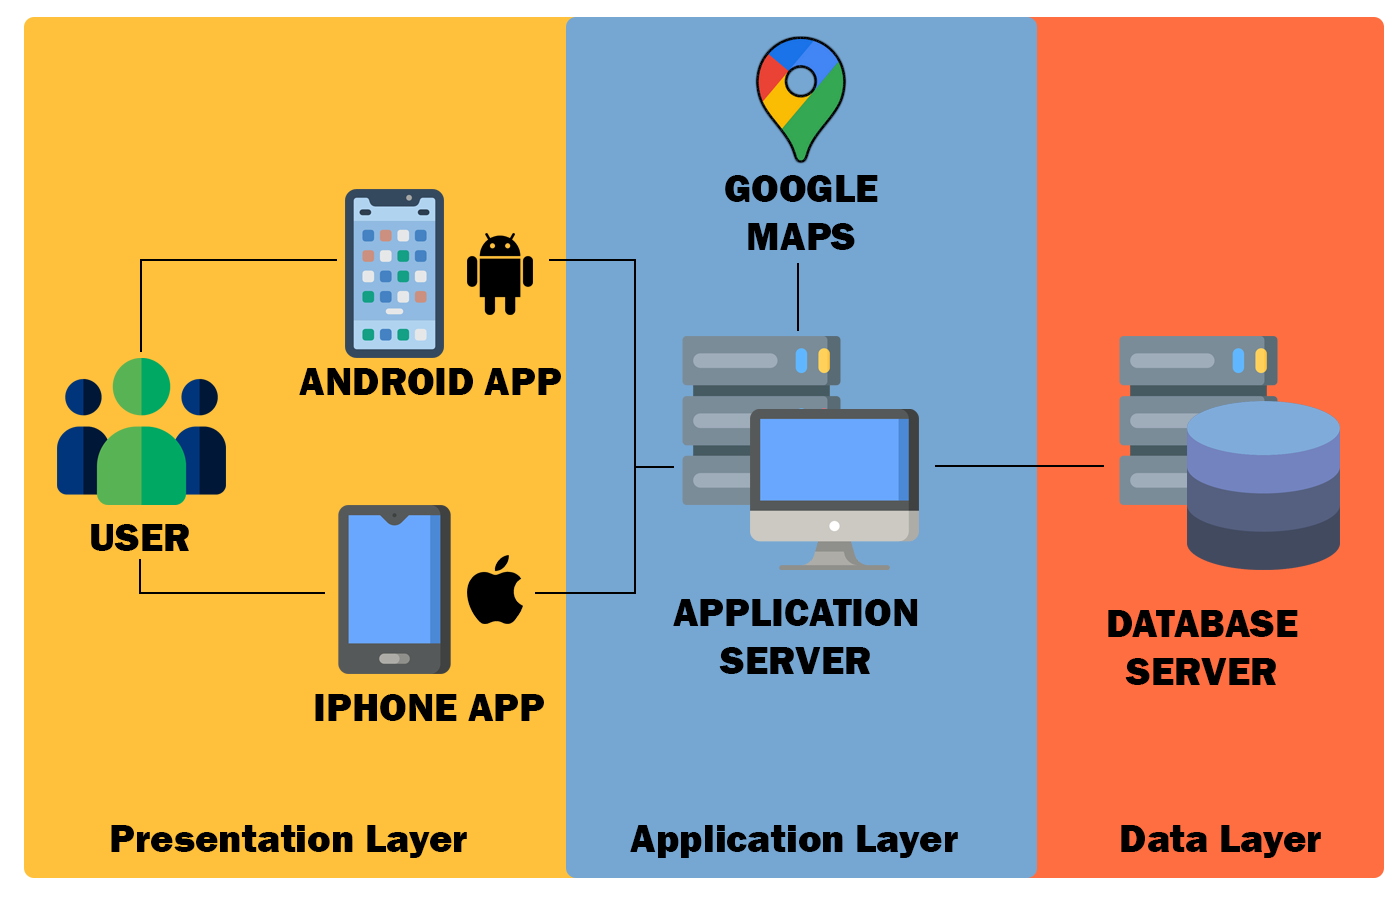
\includegraphics[width=\textwidth]{Images/DetailedArchitecturev2}
\caption{\label{fig:detailedarch}\textbf{Detailed three-layer system architecture}}
\end{figure}


\textbf{Presentation layer} – Via application interface displays messages and system options to users, gathers input, and forwards it to the application layer. Minimal computation is done here due to thin client design. It receives the data from data layer via application layer and handles interaction with user. \newline

\textbf{Application layer} – Transfers data between presentation and data layers, handles functions in the presentation layer and arranges data from data layer that is to be forwarded to the client. Communicates with Google Maps API to gather user’s current location, computes necessary time variables, and sends it to the presentation layer.  \newline

\textbf{Data layer} – Stores and manages data within database, arranges received data and sends requested data. Communicates only with the application layer. Responsible for computing the data that is only in the database.  \newline

  

Most of the additional variables, like estimated wait time and queueing is done within the data layer through the database. The data is calculated in real-time and stored directly into the database, so it is accessible to every client who requests it, with the application layer just being responsible for the data transfer. Since there are no user accounts in the application, all sent data is independent and there are no private variables for certain users (other than store managers of different stores). This improves security and privacy since no personal or vulnerable data is stored within the database. Nearly every piece of information is available to everyone, which improves speed and simplicity of the whole system due to not having to check user information by using ID tokens or some other technique. 

\newpage 

\subsection{Component view}
\label{sec:componentview}

\hspace{\parindent}In this section, a more thorough and detailed view of all of the main components is displayed. Since a lot of the work is being done in the application server part on the server, we mostly focused on that part to give a precise sketch of how some smaller parts of the system are connected and in which directions they communicate. As you can see in the component diagram, it is a very complex structure containing multiple major components and interfaces, external service, and several sub-components that are operating under one of the major ones. MobileApp and Database components are simplified and are not shown in great detail. \newline

\textbf{Component list:}
\begin{itemize}
\item DBService
\item Director
\item RequestManager
\item LoginManager 
\item StoreSelectionManager 
\item StoreManager
\item TicketService 
\item QueueService 
\item ScheduleService
\item DistanceService 
\item BookAVisitService
\item EnterService 
\item ExitService 
\item AndroidApp (external) 
\item IPhoneApp (external)
\item DB (external) 
\item GoogleMapsService (external) 
\end{itemize}

\newpage
\begin{figure}[!h]
\centering
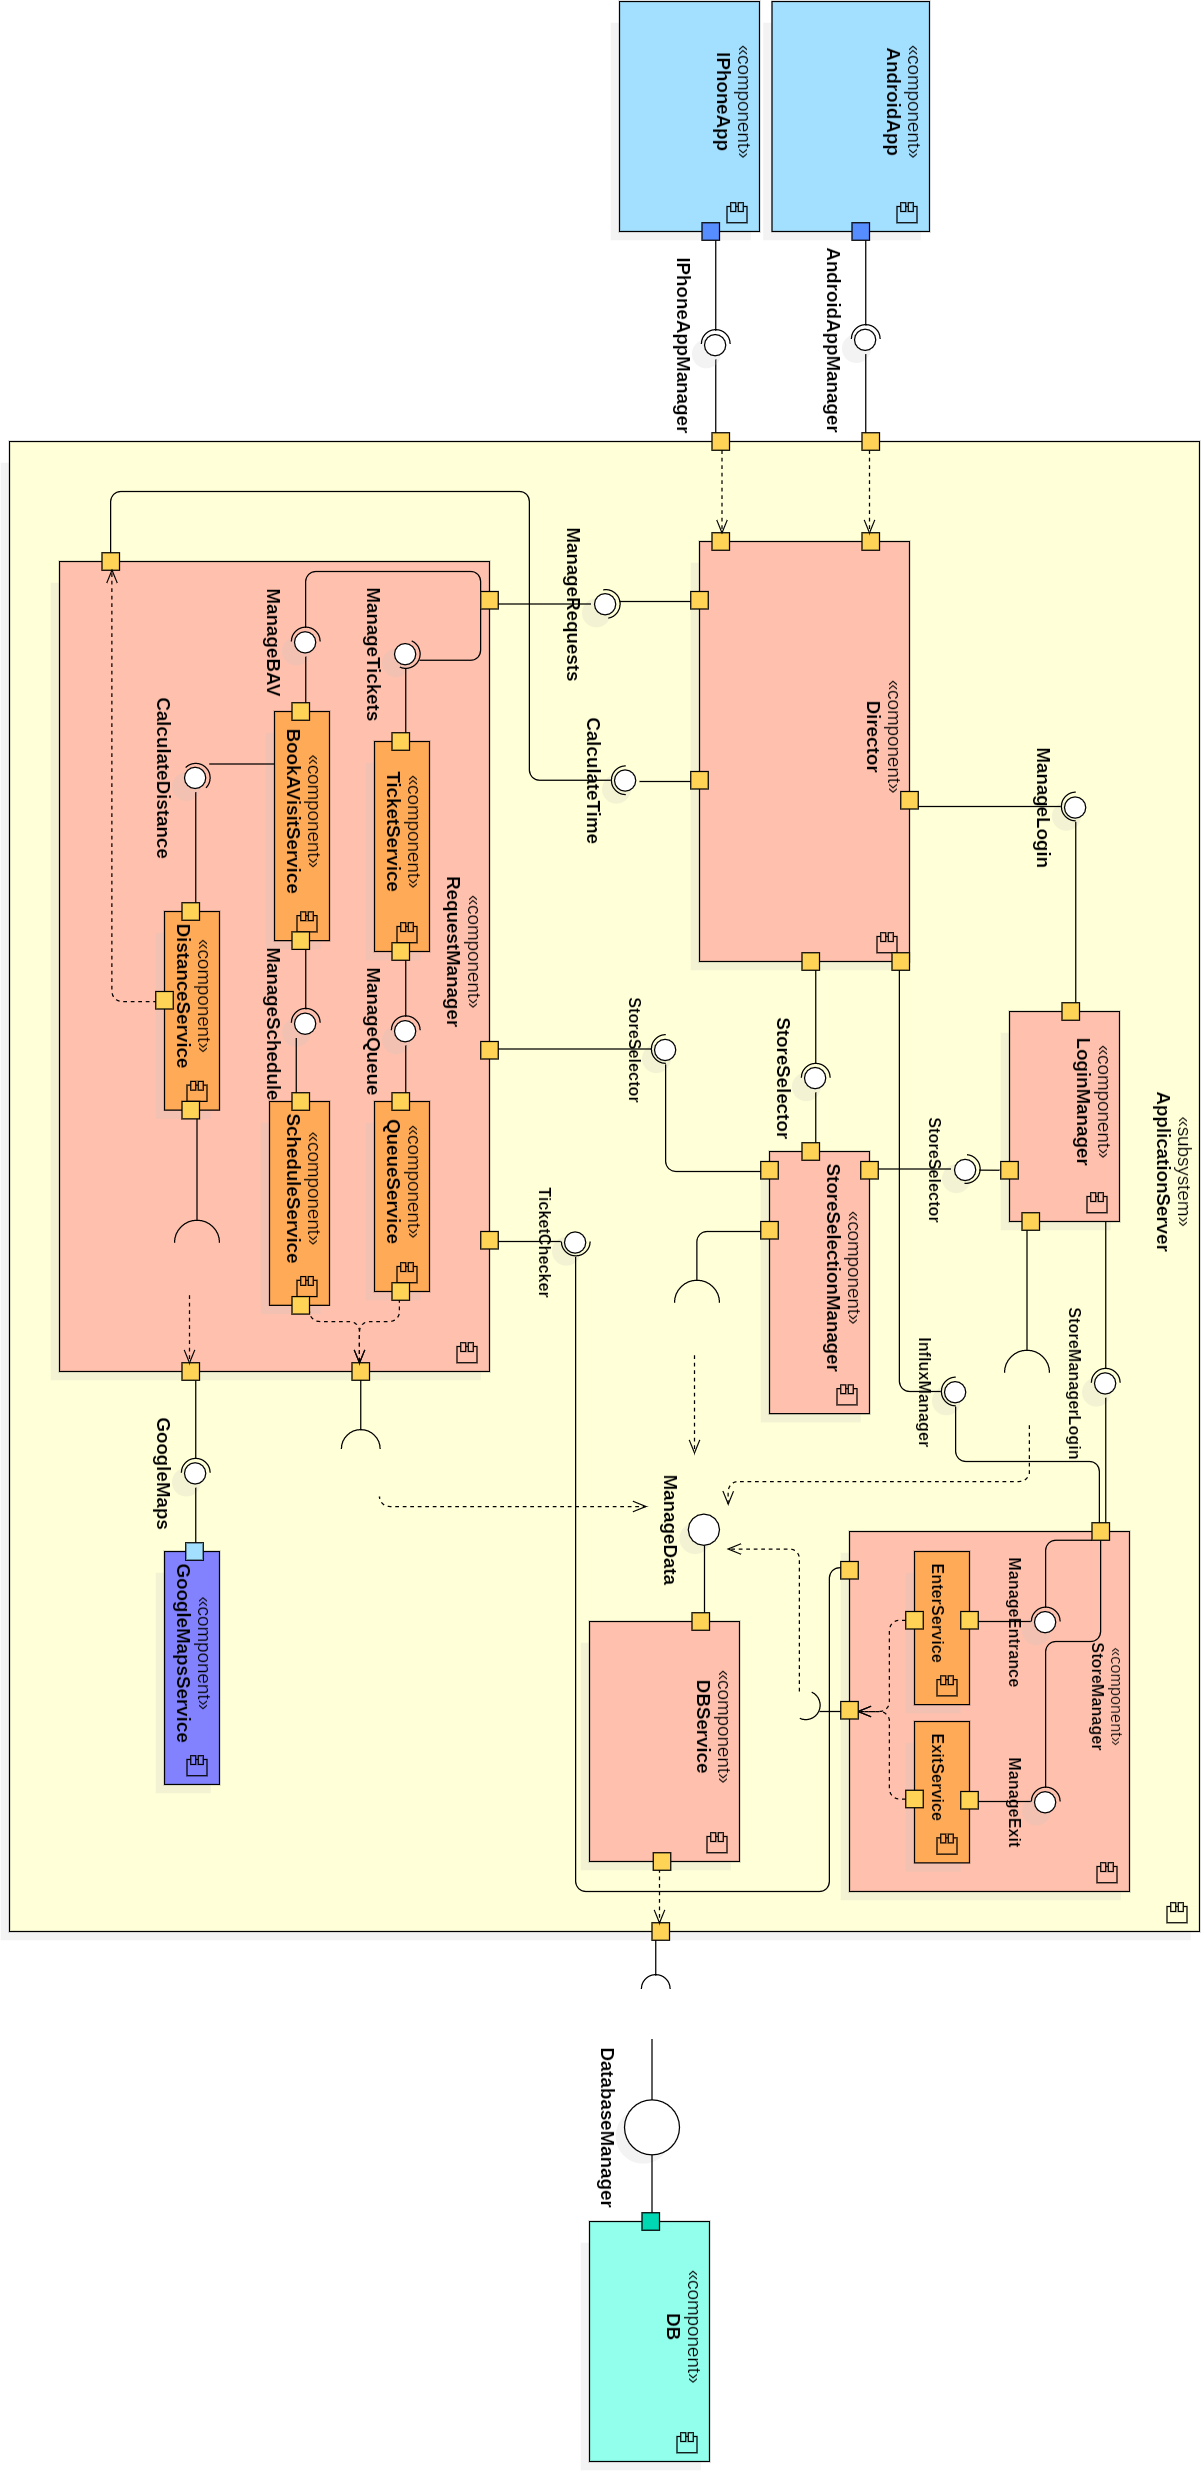
\includegraphics[width=0.65\textwidth]{Images/ComponentDiagram1v4Vert}
\caption{\label{fig:componentdiagram1}\textbf{Main component diagram}}
\end{figure}

\newpage

\begin{itemize}
\item \textbf{ApplicationServer} is one of the three major subsystems that hold the whole application logic of the system. It gathers the input from the Android and iPhone apps, does the calculation, and then transfers the data to the database while taking from it what is needed and getting it back to the phone applications in order to display it to the user. Both PhoneApps and Database are external components that are not part of the application server and the communication to them is done through sockets. The main component of the application server is Director which organizes requests from the phone apps and redirects them to other components that are dedicated to a certain request. Another bigger component is RequestManager which has several subcomponents that are explained in detail further in the text.  

\item \textbf{Director} is in charge of handling requests that are coming from the user via phone app and redirecting them to dedicated components. It is directly connected to the LoginManager, StoreSelectionManager, and RequestManager, and also indirectly connected to the StoreManager and DBService, which leads to Database. Director is also responsible for getting the return information back to the user, such as data from Database, confirmation messages, error messages, and other alerts that might be useful to the user. It is the most important part of the application server because if it fails, no messages or data can go either way.  

\item \textbf{LoginManager} is shown in the simplified form due to its simplicity, as only store managers of the stores will be using this component, since users do not have accounts and therefore do not need to login. It checks the input data username and password with the corresponding data in Database and is responsible for logging in a store manager into their store's account if the credentials are valid. It is then connected to the StoreManager via StoreManagerLogin interface. 

\item \textbf{StoreSelectionManager} is also shown in simplified form since it only features a single information that is a certain store with its name and address. When the selected store's ID is found in Database it is transferred to the RequestManager which then handles its requests and retrieves data from Database based on the ID. Because of that, to emphasize the connection of those two components, another socket has been added which directly connects StoreSelectionManager to the RequestManager.  

\newpage

\item \textbf{RequestManager} is the most complex component of the subsystem as it has five additional subcomponents. Two main functions of the application are "Request a ticket" and "Book a visit", which have their own respective services inside RequestManager. Depending on the request, QueueService and ScheduleService are activated, which then communicate with Database to send or gather additional information about the future or the current situation in the certain store (which is known via the StoreSelectionManager). If the "Book a visit" request is received, and location services are enables on the user's device, additional service called DistanceService is activated. It generates a request to the external component GoogleMapsService in order to calculate the distance from the user to the store and get the estimated time needed for the user to get there in order to arrive at a proper time in the schedule. Calculated data does not go to Database but rather goes directly back to the Director which then forwards the data to the user, since this information is based on current variables and is not something that can be reused by other users, so there is no need to put it inside the database.  

\item \textbf{StoreManager} is a component that is only used when a store manager of a certain store logs in to their account. From there, they can control the influx of people to the store, scanning and validating tickets as well as sending a signal to Database whenever a customer exits the store. It contains two services, EnterService and ExitService. EnterService concludes whether a scanned ticket is valid or not, and ExitService sends the signal to Database when a customer exits the store and also keeps track of the customer limit in a store. 

\item \textbf{DBService} is a service that does all the communication with Database. It sends all the data requests to DatabaseManager, which then access Database, and then receives the requested information back in order to return it to other managers within ApplicationServer. It basically does the same work as Director component, but talking to the database server subsystem rather than the phone app subsystem.
\end{itemize}


\newpage
\subsection{Deployment view}
\hspace{\parindent} In this section we'll touch on the architecture of the whole system in more detail, which is demonstrated with the deployment diagram. The most important components are shown as artifacts and nodes. They represent the physical deployment of software artifacts. Physical hardware is represented by nodes (cuboid) while software is represented by artifacts (rectangles with sheet icon in the upper right corner). We're also following three-layer design in this diagram, with presentation layer being on the left, application layer in the middle, and data layer on the right.   

\begin{figure}[!h]
\centering
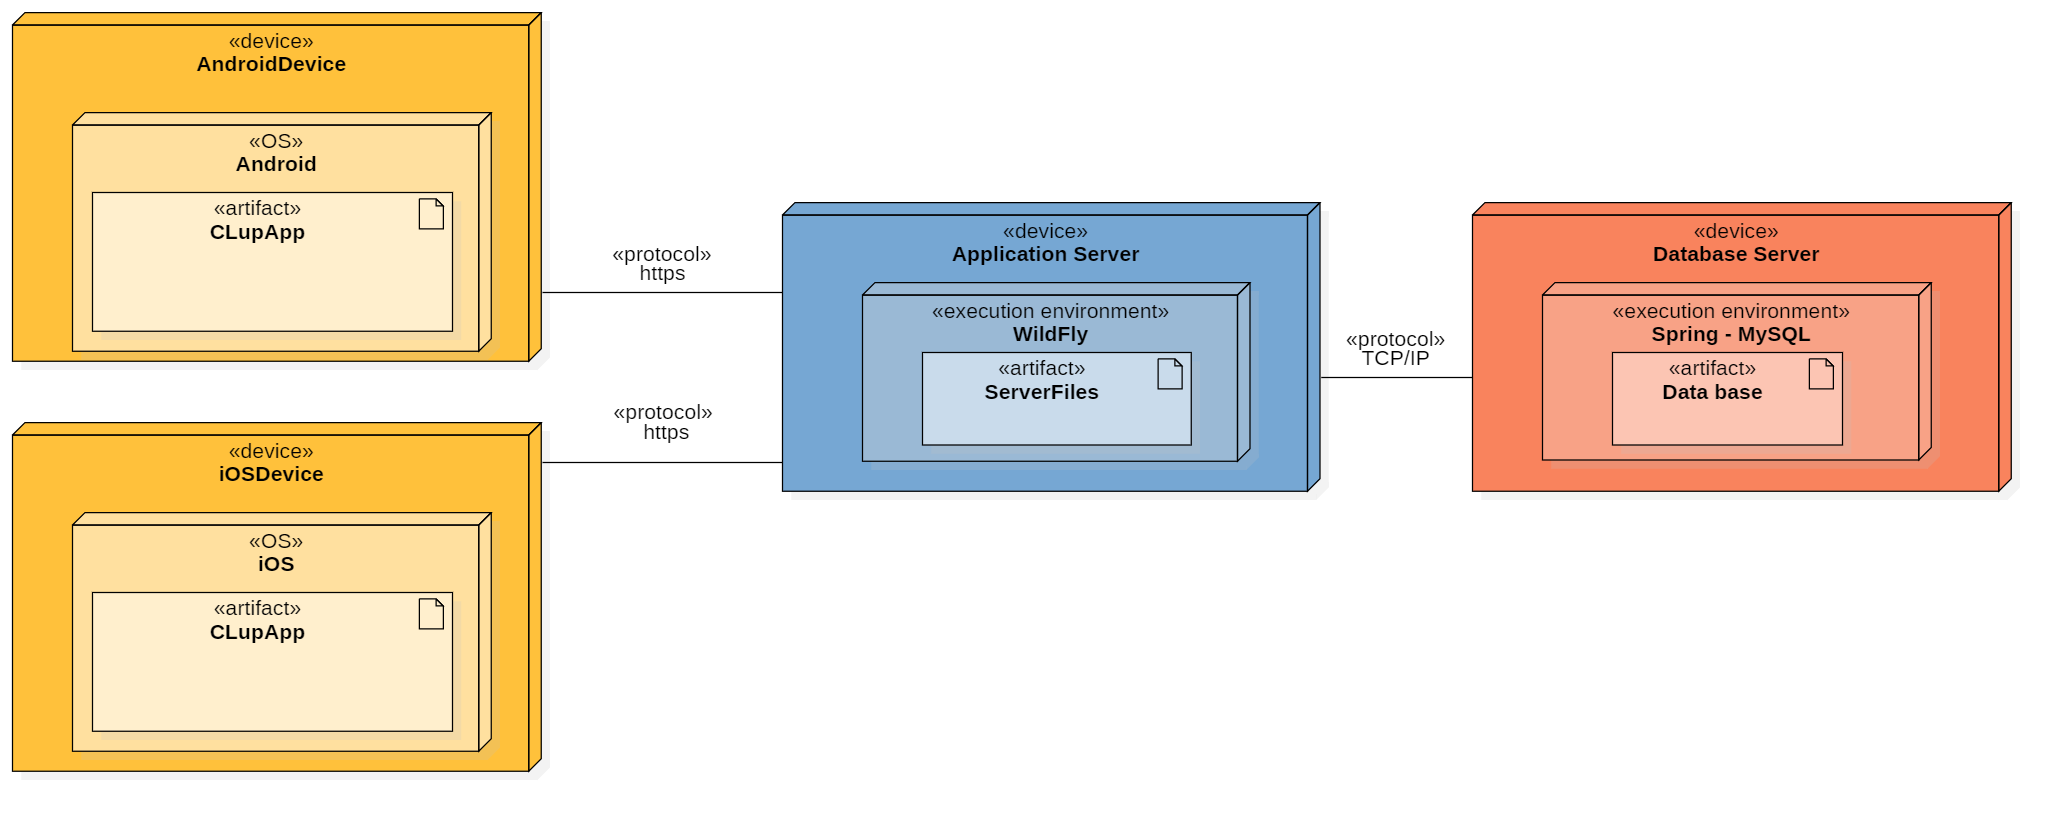
\includegraphics[width=\textwidth]{Images/DeploymentDiagram1v2}
\caption{\label{fig:deploymentdiagram}\textbf{Deployment diagram -  System architecture}}
\end{figure}


\textbf{Presentation layer} is consisting of two nodes that represent Android and iOS devices. Notice that there is no computer device which is usually common, since there is no version on the app that can be run natively on the computer or through a browser.   

  

\textbf{Application layer }is consisting a single note which represents an application, where most of the computation and application logic is being done. This layer is connected to the presentation layer via HTTPS protocol, and via TCP/IP to the data layer.  

  

\textbf{Data layer} consists of a single node which represents database server. This node is not directly connected to the presentation layer but can only communicate with the application layer.  

  

Nodes and artifacts explanations take on certain components in a bit more detailed manner. Explanations can be found in next part of this section.

\newpage

\textbf{Android and iOS devices} are both supported by CLup app, unlike the computer version, which is nonexistent due to the ticket scanning system being only available on portable devices (like tablets and phones). These platforms have operating systems that natively support running of the CLup app. The communication with the application server is being done over HTTPS protocol, which is a secure version of the HTTP protocol, over which most of the Internet traffic is going through. HTTPS is fast and very simple, allowing app requests to hastily and securely arrive to their destination.  \newline

\textbf{CLup App} is an application that is being run on of the two previously mentioned systems. It is an artifact that should have no functional differences between two versions. Even though the language and the way the app is made and deployed on these devices is different, they should offer exactly the same customer experience. \newline

\textbf{Application server} is a hardware node that is used to run the application part of the system. Our recommended execution environment is WildFly, which is a Java EE application server that consists of the application logic and components mentioned in the previous chapter. As an artifact, it has server files that are needed to run it and connect it to different parts of the system. As mentioned before, it uses TCP/IP to connect and share data with Database server.  \newline


\textbf{Database server} is a hardware node that is used to run the database needed for storing all the necessary information about the application. Desired technology to use is Spring Boot with MySQL database, which allows for simple and effective data management and delivery. Database communicates with the application server using JDBC API.    \newline

\newpage

\subsection{Runtime view}
\hspace{\parindent} In the following section sequence diagrams that represent use cases from RASD are shown and explained in detail. Since many use cases are connected and can be placed on the same diagram to better showcase the connection between the components and flow, we have created only three diagrams to represent nine use cases. Also, we have only touched those parts of the system that have to do with the application and the system itself, not displaying real-life scenarios that don't use application.  

 
Components have the same color as in the  \textbf{\hyperref[fig:componentdiagram1]{main component diagram}} which should make things easier to follow.  

\subsubsection{Book a visit}


\begin{figure}[!h]
\centering
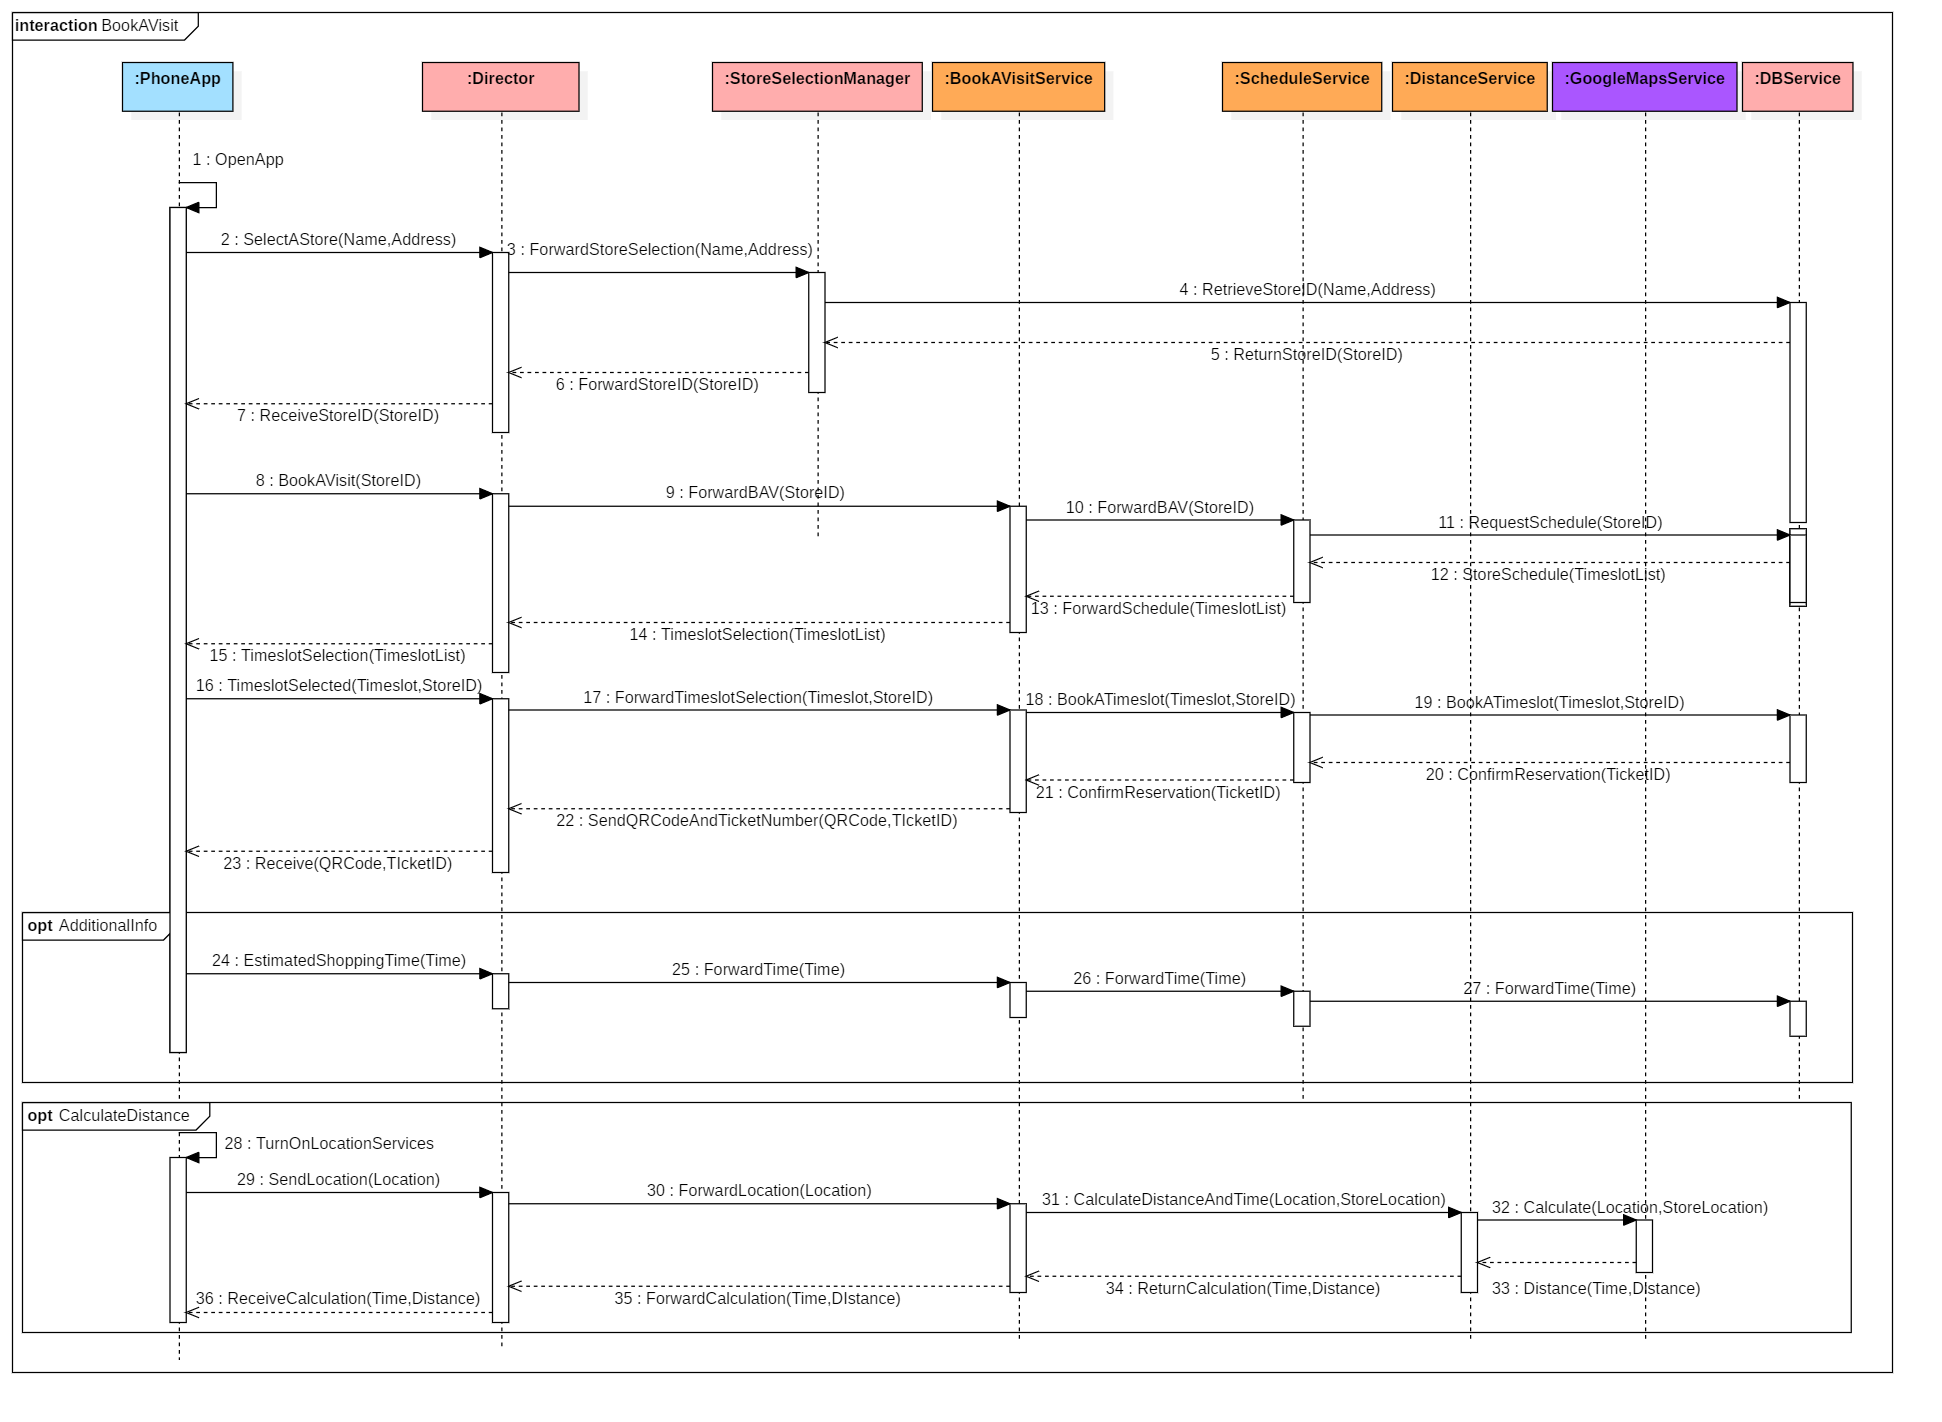
\includegraphics[width=\textwidth]{Images/SequenceDiagramComponents1_BookAVisit}
\caption{\label{fig:seqdiagram1}\textbf{Sequence diagram 1 – Book a visit}}
\end{figure}
\newpage

This diagram consists of the following components that are represented with a lifeline: PhoneApp, Director, StoreSelectionManager, RequestManager (which is represented with its services BookAVisitService, ScheduleService, and DistanceService), GoogleMapsService, and DBService.  

  

The diagram shows one of the basic functions of the app, which is booking a visit to the store at a certain time and optionally, adding estimated shopping time and calculating distance from the store.  

  

Every diagram including this one starts with the app opening and store selection. Store is selected by choosing a store from a list which contains store's name and address. This selection is forwarded through Director to the StoreSelectionManager, which then asks for the StoreID and details from the DBService. Every request that comes to the DBService is forwarded to Database which is not shown in these diagrams. After fetching the data from Database, DBService returns the StoreID which goes all the way back the same way to the PhoneApp.   

  

The user then proceeds with using Book a visit feature. The feature is requested along with a StoreID all the way to DBService, using Director, BookAVisitService, and ScheduleService, with the latter two being a part of the RequestManager which then retrieves a schedule for that specific store with a list of available timeslots. User then receives the list and picks his timeslot, which starts the return to Database.  

  
After DBService has gotten confirmation and a ticket from Database, it transfers the confirmation along with the QR code and a ticket back to the PhoneApp.  
  
There are additional two actions that the user can perform but doesn't have to. Both actions aim to improve user experience and better approximate waiting time.  

  

One of the actions is user entering estimated shopping time, which is then forwarded directly to database. Database stores the data and uses it when other users request a ticket, in order to approximate their waiting time.  

No additional confirmations are returned to the user, because they are not needed.  

  

The second optional action is calculating distance from the user to the store. The system is capable of calculating both distance in meters and in time it takes to get there, using the Google Maps API. If the user has enabled location services and chosen this option, request is sent to BookAVisitService, which forwards it then to DistanceService and GoogleMapsService. After Google Maps API has calculated the distance, it is returned immediately to the user, without going to the database, since this information is used only one time for a specific user, and it is not reusable, which makes it unnecessary to hold in the database.  
\newpage

\subsubsection{Retrieve a number }


\begin{figure}[!h]
\centering
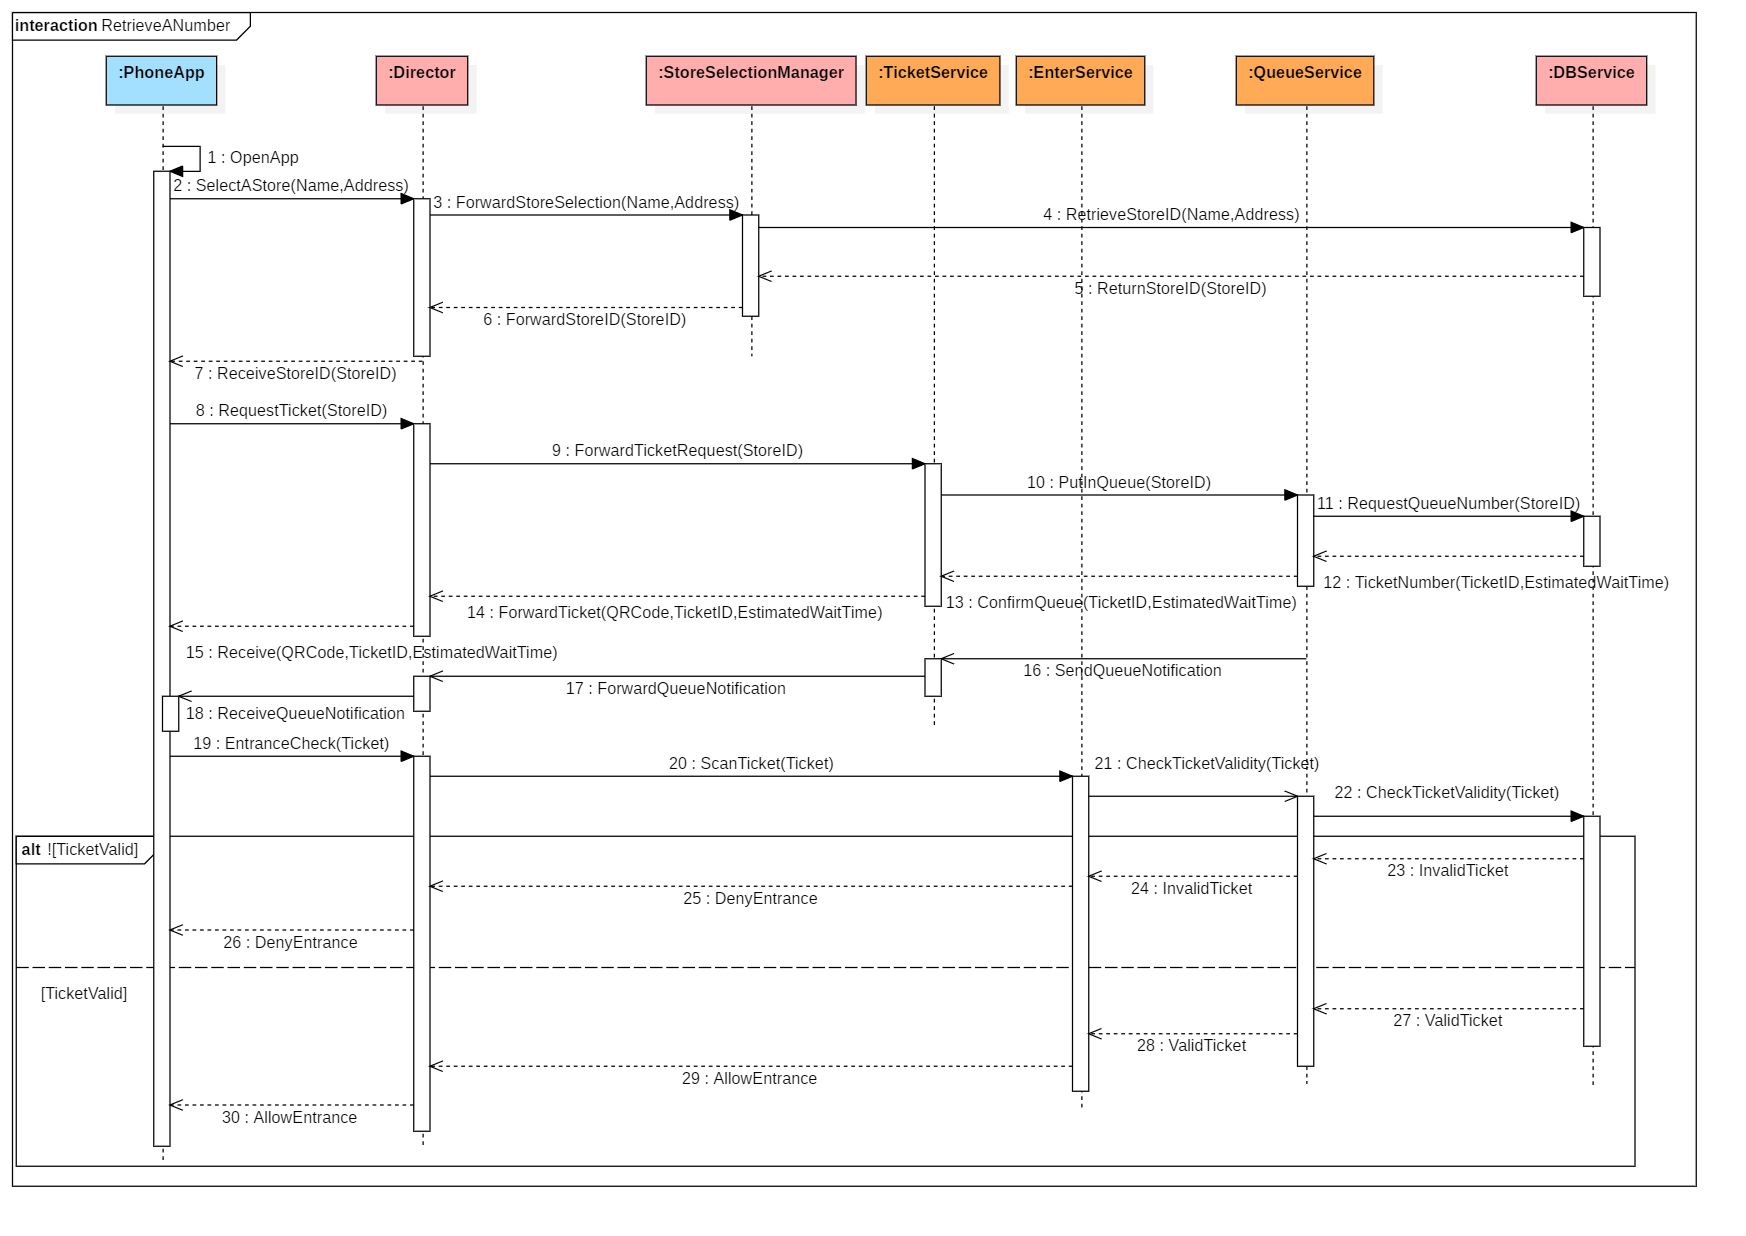
\includegraphics[width=\textwidth]{Images/SequenceDiagramComponents2_RetrieveANumber}
\caption{\label{fig:seqdiagram2}\textbf{Sequence diagram 2 – Retrieve a number}}
\end{figure}

This diagram consists of the following components that are represented with a lifeline: PhoneApp, Director, StoreSelectionManager, RequestManager (which is represented with its services TicketService and Queue Service), StoreManager (which is represented with its service EnterService), and DBService.  

  

The diagram shows one of the basic functions of the app, which is requesting a ticket for entering the store immediately (or in a very near future depending on the queue), as well as the process of ticket validation at the store's entrance.   

  

The process is for the most part very similar to the Book a visit diagram above but uses some different services. Also, the latter part of the diagram can also be applied to the Book a visit diagram, but it has been omitted from there to put the emphasis on different components and communication between them. However, everything from the message number 16 to the message number 27 on this diagram is also happening when entering a store after getting the ticket with "Book a visit" feature.   

  

After opening the app, the user selects a store in the same way as in the previous diagram. The request goes through Director and StoreSelectionManager before getting to the DBService which gets the StoreID from Database and returns it to the user.  

  

The process of requesting the ticket starts with a user generated request. The request goes through Director which then forwards it to TicketService. TicketService generates a ticket and forwards it to QueueService which puts it in the queue. DBService updates the current data for the store, and the ticket with a number and a QR code is then returned to the user.  User also receives approximated wait time he is going to have to wait in queue before being able to enter the store. 

  

When the user gets the notification that it is his time to enter the store, he presents the ticket to the store manager, who scans it. The ticket is then being checked by EnterService and QueueService. Depending on the validity of the ticket, the user is allowed or denied entrance to the store.   


\subsubsection{Store manager login}


\begin{figure}[!h]
\centering
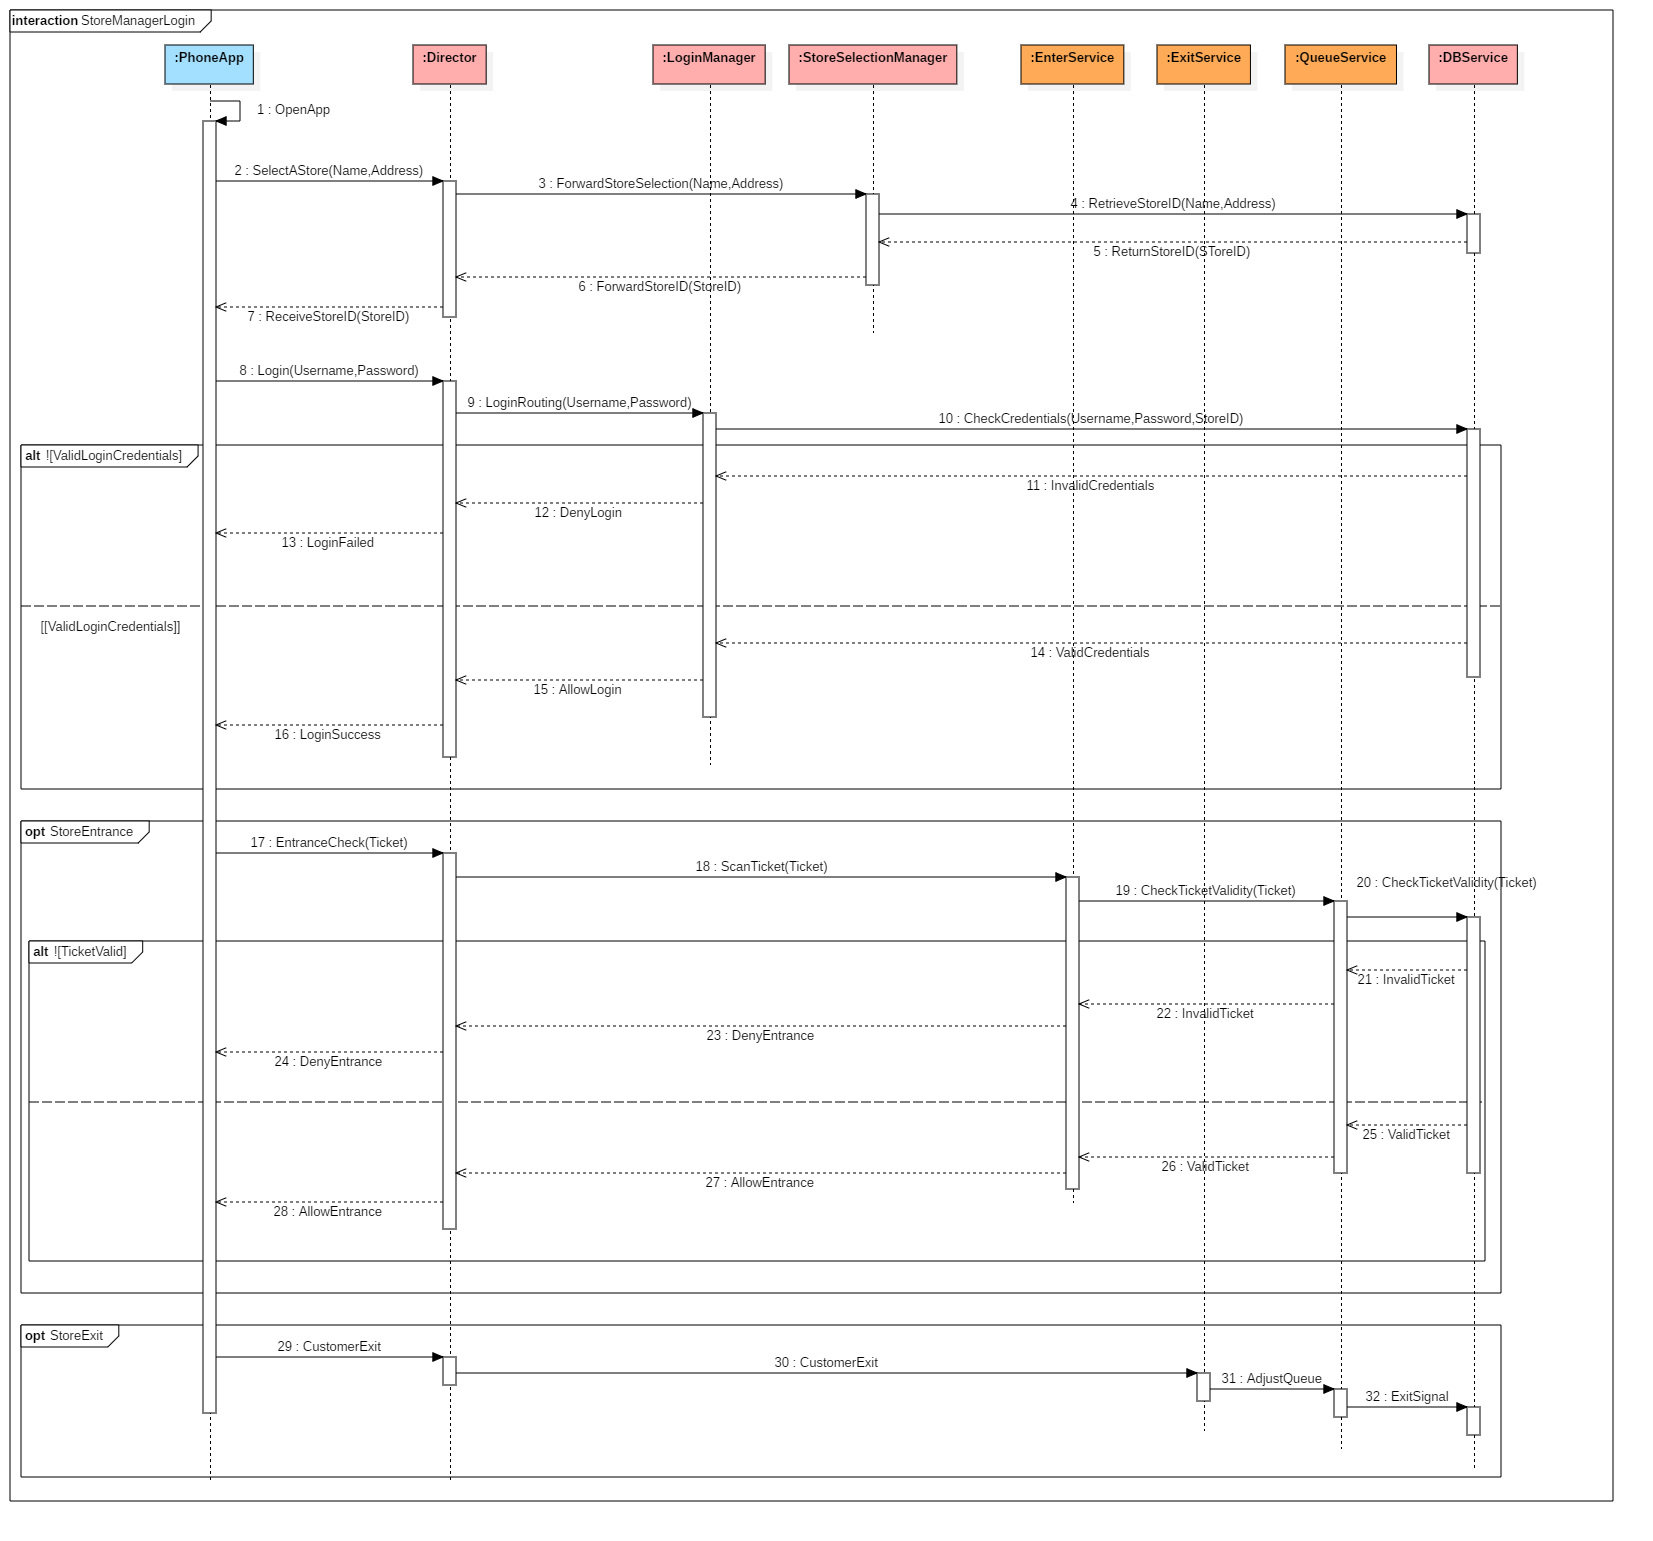
\includegraphics[width=\textwidth]{Images/SequenceDiagramComponents3_StoreManager}
\caption{\label{fig:seqdiagram3}\textbf{Sequence diagram 3 – Store manager login}}
\end{figure}
\newpage

This diagram consists of the following components that are represented with a lifeline: PhoneApp, Director, LoginManager, StoreSelectionManager, RequestManager (which is represented with its service Queue Service), StoreManager (which is represented with its services EnterService and ExitService), and DBService.  

  

This diagram shows the whole process of the store manager login and app usage when controlling the influx of customers to the store. The diagram consists of three parts – store manager login, customer entrance, and customer exit.  

  

The first part begins with opening the app and selecting a store. The process of selecting a store is exactly the same as in previous two diagrams, so that part will not be explained in detail.  

  

Afterwards comes the store manager login screen. Store manager must provide his username and password (which is given to him after the registration of the store that is done manually by the admins and creators of the app). Request goes through Director and LoginManager all the way to DBService, which checks the credentials in Database, and based on their validity, either allows the login and logs in the store manager or denies the login and returns the error message.  

  

The second part of the diagram begins every time a customer wants to enter the store. Store manager scans their ticket. The ticket information is then sent to EnterService and to QueueService. After checking the ticket validity there and updating Database, the ticket is either valid or invalid, which either allows or denies the entrance to the store for the customer.   

  

The third part of the diagram is much simpler – every time a customer exits the store, the store manager just sends the signal by pressing the button on the app. That signal is then sent to ExitService and to QueueService. The queue and the database are updated. No return signals are given to the store manager after that action.   


\newpage

\subsection{Component interfaces}

\hspace{\parindent}The complexity of developing a mobile application encourages the engineers to split the paramount task into smaller subproblems, or components. Each component is then encapsulating a certain part of the applications function, and communicating with other components through interfaces. The use of interfaces enables the developer of a component to be unaware of the concrete implementation of other components, but just know the syntax of their method calls. 

This section gives a thorough overview of the systems interfaces, divided by components they belong to. It is important to note that the interfaces and their methods proposed in this section, do not necessarily represent the exact written counterparts in the implementation, but offer a basic guideline of the component communication. \newline

\textbf{General interfaces: }
\begin{itemize}
\item AndroidAppManager
\item iPhoneAppManager 
\item RequestTicket 
\item EntranceCheck 
\item GiveTicket 
\item InformUserToEnter 
\item CheckTicket 
\item CalculateTime 
\item ManageRequests 
\item StoreSelector 
\item InfluxManager 
\item ManageLogin 
\item ManageData 
\item DatabaseManager 
\item GoogleMaps 
\item ManageTickets 
\item ManageBAV 
\item CalculateDistance 
\item ManageSchedule 
\item ManageQueue 
\item StoreManagerLogin 
\item ManageEntrance 
\item ManageExit 
\item TicketChecker 
\end{itemize}

To begin with, the application on the users phone communicates with the system through AndroidAppManager and IPhoneAppManager interfaces, according to the type of the users OS. They enable communication between ApplicationServer, or more specifically, the Director component, and the smartphone application. Depending on the type of the user, the interface offers all methods for the interaction with the system. 

For example, upon the push of a button in the UI, the application invokes RequestTicket method on the Director to propagate the request. Similar to that, an application of a store manager can invoke CheckTicket method on the Director, to propagate the specific request to ApplicationServer. \newline
 

The systems' main global component, ApplicationServer, is divided into smaller core components Director, GoogleMapsService, LoginManager, StoreSelectionManager, DBService, StoreManager and RequestManager. The communication between the core components is also done through interfaces. 

For the Director to propagate users requests, RequestManager offers methods contained in ManageRequests interface. Other than that, the two components also communicate to calculate wait time through CalculateTime interface. 

Furthermore, Director component communicates with LoginManager and StoreSelectionManager components. For LoginManager, it does so through a ManageLogin interface, which enables the propagation of the credential check used when a store manager accesses the application. For StoreSelectionManager, it uses methods offered by StoreSelector interface. \newline

To enable users to choose between the stores using the CLup system, StoreSelectionManager also offers StoreSelection interface, used by LoginManager for store managers and RequestManager for store customers. 

The calculation of the distance between the user and the store is done with the help of Google Maps. To implement that, GoogleMapsService offers a GoogleMaps interface to RequestManager. Upon gathering information, RequestManagers subcomponents BookAVisitService and DistanceService perform the distance calculation through CalculateDistance interface. \newline

Depending on the type of the user request, RequestManager further branches into different subcomponents. TicketService and QueueService encapsulate functions needed to perform the get in a virtual line function, and BookAVisitService and ScheduleService serve to carry out the "Book a visit" function of the system. For communication between the Director and RequestManager, the former uses ManageTickets and ManageQueue interfaces, whereas the latter uses ManageBAV and ManageSchedule interfaces. \newline

To physically manage store entrances and exits, the CLup system also offers a specific interface for the store managers. The logic behind that interface is contained in StoreManager component. The component communicates with LoginManager through StoreManagerLogin interface, to execute logins of the store managers. This design choice improves upgradeability for future requests and different users. Furthermore, StoreManager component also communicates with DBService to persist data through ManageData interface. Before persisting, the data is handled by the subcomponents EnterService and ExitService through ManageEntrance and ManageExit interfaces. To connect the full circle of the system function, through TicketChecker interface, offered by RequestManager, StoreManager can control the influx of the customers. \newline


Lastly, in order to persist the applications data, DatabaseManager interface is used. The interface enables the application server, or more precisely, DBService component, to invoke methods to write data to, or read data from, Database. DBService itself, offers ManageData interface to all other subcomponents of ApplicationServer to connect them to Database. \newline

\begin{figure}[!h]
\centering
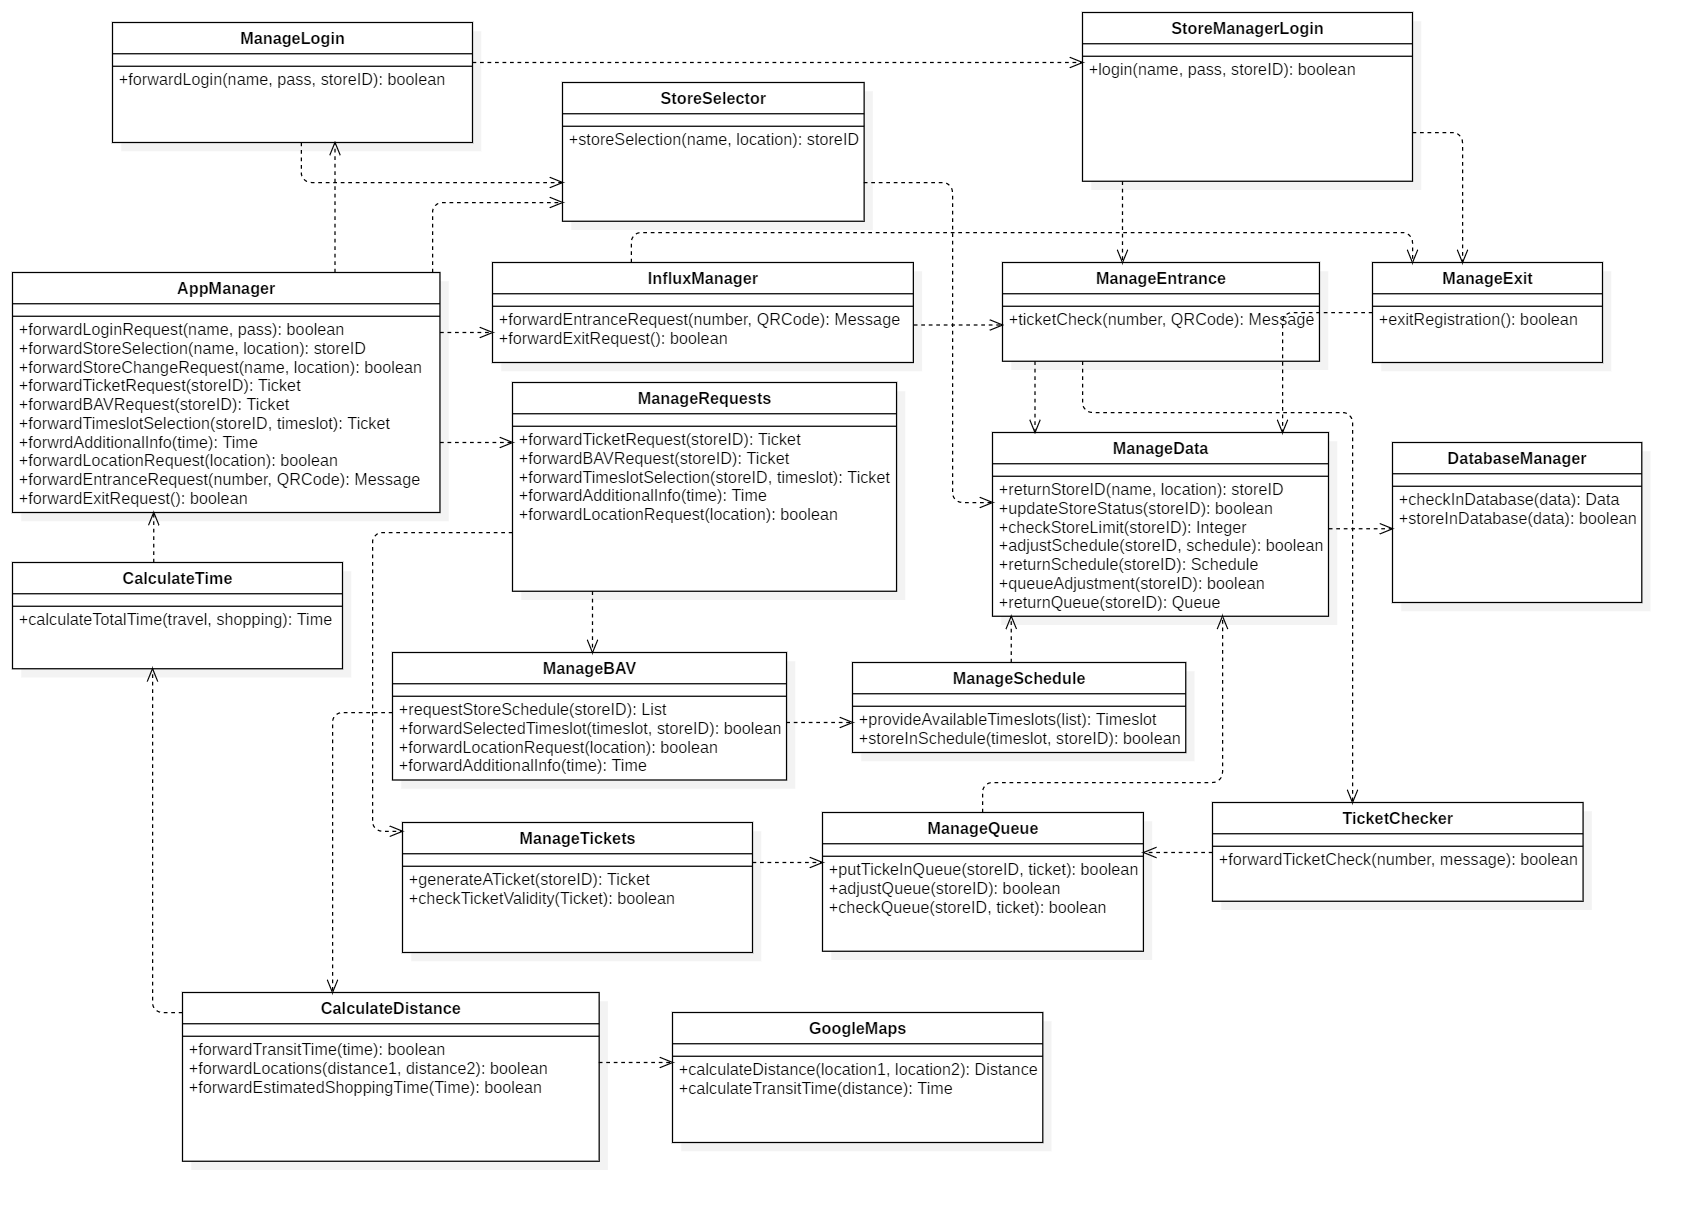
\includegraphics[width=\textwidth]{Images/InterfaceDiagram}
\caption{\label{fig:interfacediagram}\textbf{Interface diagram}}
\end{figure}

\newpage
\subsection{Selected architectural styles and patterns}

\begin{figure}[!h]
\centering
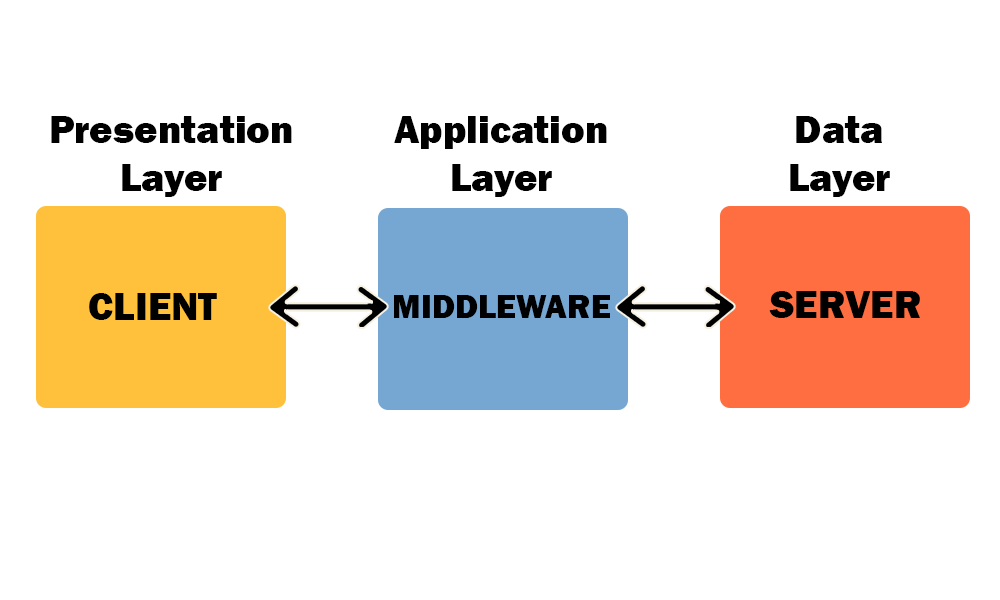
\includegraphics[width=\textwidth]{Images/ThreeLayers}
\caption{\label{fig:arch}\textbf{Three-layer system architecture}}
\end{figure}

To develop the full system, a three-tier client-server architecture will be used.  The choice is encouraged by the popularity of the model, and its valuable aspects such as modularity, scalability or abstraction. The three layers in the three-tier architecture are: presentation layer, application layer, and data layer. By dividing system artifacts in three different layers and enabling mutual communication with abstract interfaces, we hide unnecessary information and improve testability of each single layer. To communicate, the server waits for the clients requests, and upon a request, it extracts data from the database, processes it, and serves it to the client.  

Depending on the needs of the system and the work done locally on the client, the client can be thin or thick. For the CLup system, a thin client design is a much better fit, since the calculations can easily be done on the server, and the application has to be usable by all smartphones, even the older ones. The data processed by the server can then be presented to the client device. \newline

Basic software design practices such as modularity and the use interfaces will help greatly with the development, testing and further improvement of the application. Dividing the code in concise modules encourages reusability, and enables extensive upgradeability. Additionally, having functional modules makes component testing possible and quick. Abstraction in code, done through the use of interfaces enhances all the aforementioned effects and relieves the developer of the knowledge and complexity of all components outside his scope. \newline

 

\begin{figure}[!h]
\centering
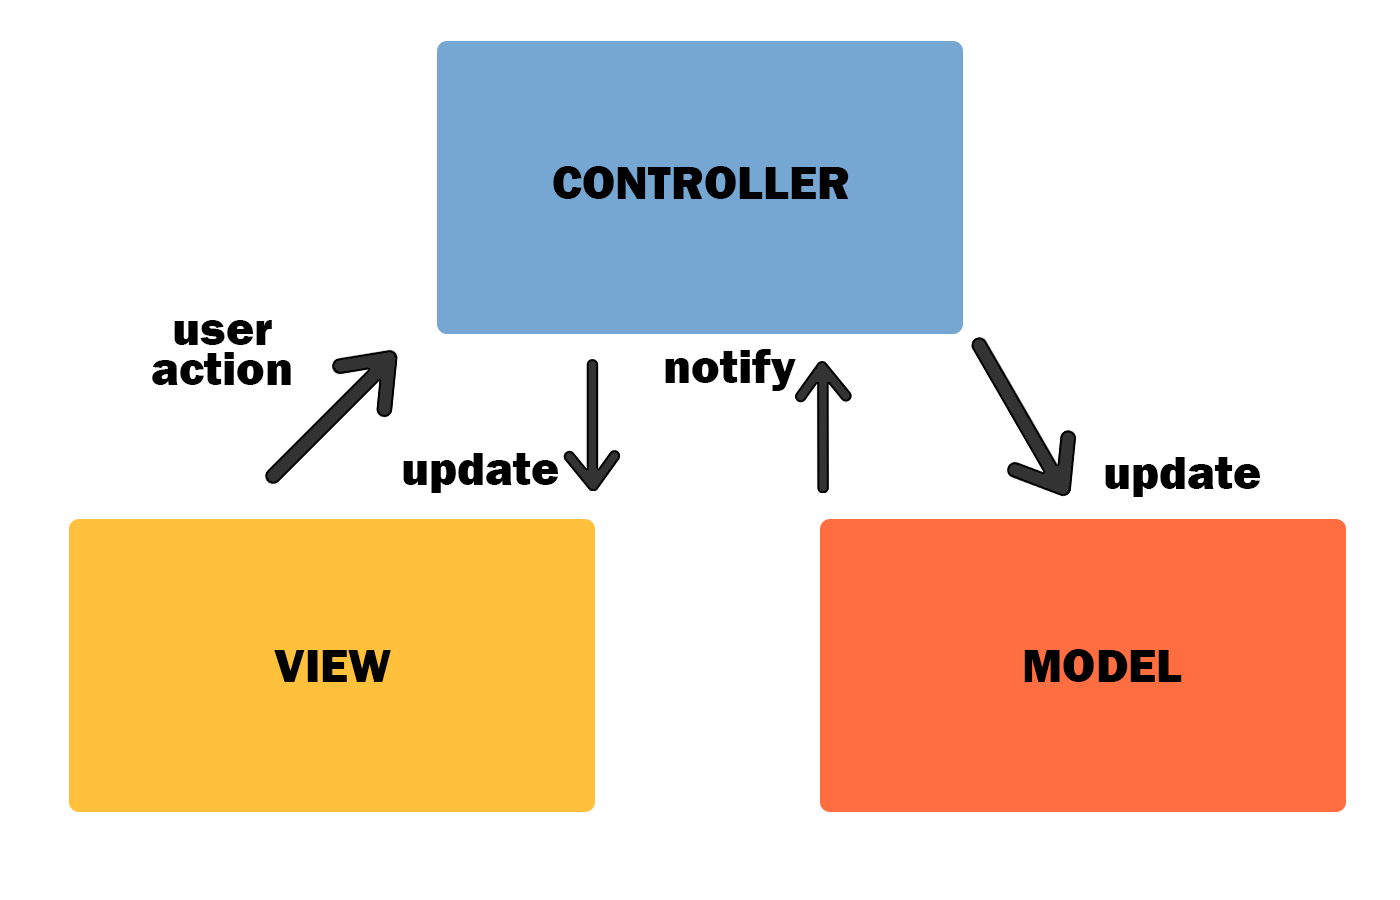
\includegraphics[width=0.9\textwidth]{Images/MVC}
\caption{\label{fig:mvc}\textbf{Model-view-controller}}
\end{figure} \newpage

 

We would also like to take advantage of the MVC(Model-View-Controller) global design pattern. The pattern is widespread in the software engineering community because of its scalability and simplicity, and provides a perfect base for our application. The Model component is the main component of the pattern in charge of the business logic. The View component controls the user interface, and the way in which information is represented. And the Controller component acts as a bridge between the Model and the View. It accepts data from, and creates instructions for the Model or the View. \newline


To persist data like store enter and exit times, the system must be able to communicate with a database. DAO(Data Access Object) design pattern acts as an interface and makes that possible. For example, if written in the Java language, JDBC API will be used as DAO. 

 

Main communication protocol used in the system is HTTPS. It provides a simple, popular, and secure connection for message exchange. It is also important to note that to use third-party software, we need to use specific protocols. In the case of GoogleMaps, we need to use the REST API. \newline

 

In the end, the main software design patterns will be mentioned. Firstly, Observer/Listener behavioral pattern enables the system to subscribe to the updates of the client devices location and upon change execute new calculations. The pattern defines a one-to-many connection between objects and updates them automatically upon notification. And lastly, Bridge structural pattern is used in various places to decouple an abstraction from the implementation. In that way, components can be changed and substituted by new ones completely independently. Through aggregation and encapsulation the Bridge separates responsibilities into different classes. 
\newpage
\subsection{Other design decisions}
\hspace{\parindent}The CLup system relies on two main third party components to function properly: Database and the GoogleMaps API. Since most popular database vendors nowadays offer very similar functionalities, the database choice is left to the development team. For the needs of the system, even a NoSQL database system, like Firebase, would work. Firebase is a platform for creating applications, both web and mobile. It was founded in 2011 and is now the primary database option for application development offered by Google. It offers a real-time database, simple interfaces, and high-level security, which makes it well suited for our needs. \newline

To calculate the expected time for a customer to get to the store, the best choice is GoogleMaps API. Through the years, Google polished their map system offer and today they have a widespread, highly accurate, and easy-to-use satellite imagery and street maps. It also offers, real-time traffic conditions and route planning for traveling by foot, car, and public transport which makes it a perfect match for the needs of the CLup system.\newline 

In the end, one important design decision should be noted: to avoid security concerns with storing sensible user data in the database, the first version of the system evades user registration altogether. The scope of the system, so far, does not require the system to store such data. However, if the scope of the system grows in such a way that user registration becomes imminent, upgrade of the system built in line with this design document should not be a problem, especially since a form of user registration should already be implemented on the store manager's side. 
\newpage




